\documentclass[twoside,11pt]{article}

% Any additional packages needed should be included after jmlr2e.
% Note that jmlr2e.sty includes epsfig, amssymb, natbib and graphicx,
% and defines many common macros, such as 'proof' and 'example'.
%
% It also sets the bibliographystyle to plainnat; for more information on
% natbib citation styles, see the natbib documentation, a copy of which
% is archived at http://www.jmlr.org/format/natbib.pdf

\usepackage{jmlr2e}

% packages for fancy fonts, symbols, thm/proof environments, etc
\usepackage{amsmath,amssymb,amsthm}
\usepackage{graphicx}
\usepackage{hyperref}
\usepackage{subcaption}
\usepackage{wrapfig}

\setcitestyle{square}


% Custom colors
\usepackage{color}
\definecolor{deepblue}{rgb}{0,0,0.5}
\definecolor{deepred}{rgb}{0.6,0,0}
\definecolor{deepgreen}{rgb}{0,0.5,0}

\usepackage{listings}

% Python style for highlighting
\newcommand\pythonstyle{\lstset{
language=Python,
basicstyle=\ttm,
otherkeywords={self},             % Add keywords here
keywordstyle=\ttb\color{deepblue},
emph={MyClass,__init__},          % Custom highlighting
emphstyle=\ttb\color{deepred},    % Custom highlighting style
stringstyle=\color{deepgreen},
frame=tb,                         % Any extra options here
showstringspaces=false            % 
}}


% Python environment
\lstnewenvironment{python}[1][]
{
\pythonstyle
\lstset{#1}
}
{}

% Python for external files
\newcommand\pythonexternal[2][]{{
\pythonstyle
\lstinputlisting[#1]{#2}}}

\newcommand{\dataset}{{\cal D}}
\newcommand{\fracpartial}[2]{\frac{\partial #1}{\partial  #2}}

% Heading arguments are {volume}{year}{pages}{submitted}{published}{author-full-names}

% Short headings should be running head and authors last names

\ShortHeadings{Project CNN - COGS 185}{Thomas Astad Sve}
\firstpageno{1}

\begin{document}

\title{Advanced Machine Learning Methods \\ Project CNN}

\author{\name Thomas Astad Sve \email thomaasv@stud.ntnu.no \\
         \addr Computer Science, Artificial Intelligence\\
       Norwegian University of Science \& Technology\\
       \addr University \& Professional Studies \email ax004206@acsmail.ucsd.edu\\
       University of California, San Diego\\}

\maketitle

\begin{abstract}
  I trained a Convolutional Neural Network on GPU for classifying images using the tiny ImageNet data set. The model is built after googlenet's \cite{googlenet} architecture using the python library lasagne \cite{lasagne}, which is built on top of theano \cite{theano}. The CNN network consist of 22 layers and achived a total accuracy of 30 \% when having 100 different classes. A reduced version with 20 different classes got a total of 37 \% accuracy on the test-set. More in depth analysis would have been considered if I had more time available to test several CNN networks. I also cut the original data set of 200 to 100 classes to reduce training time as I calculated it would take me up to three days to train with the 200 classes.
  
\end{abstract}
\section{Introduction}
A common problem in machine learning is to effective representation of complex inputs such as image and video. Over the past years deep learning has proven to perform on such complex problems. 
I use Convolutional Neural Networks for image classifications on the tiny ImageNet dataset, a smaller version of the ImageNet \cite{imagenet} challenge dataset.
\section{Method}
\subsection{Model}
The model used to build the classifier is a model based on the googlenet architecture. I used the library lasagne \cite{lasagne} which is built on theano for deep learning. I also found the recipie for the model online \cite{googlenet-recipe}. The network has 22 layers where 9 of the layers is inception layers with dimensionality reductions. 
\subsection{Data Set}
Tiny ImageNet is a dataset with 120,000 labeled images into 200 different categories. The dataset is similar to the ImageNet used in the ILSVRC benchmark, known as the ImageNet challenge. The images in the tiny dataset have lower resolution and it's an smaller dataset in total. Each of the 200 categories consists of 500 training samples with a 64x64 resolution. The raw RGB pixel-values of these images areextracted and fed to the CNN network.

\begin{wrapfigure}{r}{0.5\textwidth}
  \begin{center}
    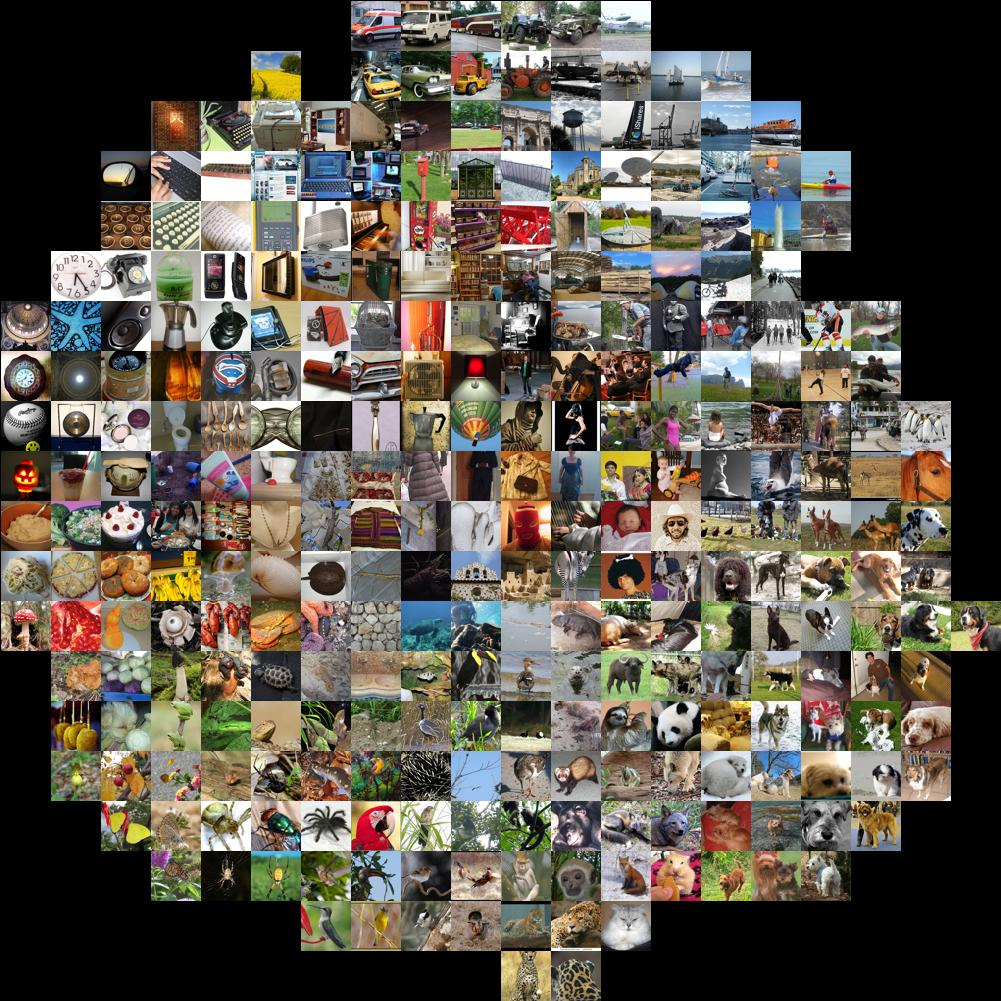
\includegraphics[width=0.4\textwidth]{images/cnn_embed_1k.jpg}
  \end{center}
  \caption{TSNE Embedding of Tiny Imagenet CNN Codes}
  \label{fig:tiny-imagenet}
\end{wrapfigure}

\section{Experiment}


\section{Results}
In order to test my program to see if it would run, I first classified a smaller version of the dataset with only 20 classes. This took around 3 hours running 500 epochs. After having confirmed everything worked with a low number of classes, I wanted to test if I could run for the whole dataset with 200 classes. Starting to train the classes with 200 classes took me around 380seconds per epoch, and I realized I would have to run for many days to complete it. I therefore decided to reduce down to 100 classes with epoch of 250. With 100 classes it now took me 190 seconds per epoch, and running 250 epochs it took me around 14 hours to complete it. I could have let the network run at 200 classes and rather reduce the layers to make the network less deep, or significantly reduce number of epochs. I chose not to do this to keep the depth of the network.

\begin{table}[!htbp]
  \centering
\caption{\label{tab:results} Shows results for running classification on Googlenet}
\begin{tabular}{| l l l l l l l|}
  \hline
  \# classes & \# training & \# validation & \# testing & \# epoch & test-loss & Accuracy\\ \hline
  20 & 6903 & 1480 & 1480 & 500 & 10.9 & 39.30 \\
  100 & 39340 & 4928 & 9835 & 250 & & \\
  \hline  
\end{tabular}
\end{table}

On epoch 50 it was actually lower than epoch 30. Looking closer at the runs, it shows that on epoch 49 and 51 it was around 28 \%, meaning it hasnt really changed since epoch 30, it just dropped a little on the actual round 50. 

\begin{table}[!htbp]
  \centering
\caption{\label{tab:results} Shows results for validation accuracy for Googlenet on tiny ImageNet with 100 classes on some epochs}
\begin{tabular}{| l l |}
  \hline
  Epoch & Val accuracy \\ \hline
  1 & 1.51 \%\\
  5 & 7.29 \%\\
  10 & 16.53 \%\\
  20 & 25.89 \%\\
  30 & 27.38 \%\\
  50 & 22.64 \%\\
  100 & \\
  150 & \\
  200 & \\
  250 & \\
  \hline  
\end{tabular}
\end{table}


\begin{figure}[!htbp]
        \begin{subfigure}[b]{0.25\textwidth}
                \includegraphics[width=\linewidth]{example-image-a}
                \caption{A gull}
                \label{fig:gull}
        \end{subfigure}%
        \begin{subfigure}[b]{0.25\textwidth}
                \includegraphics[width=\linewidth]{example-image-a}
                \caption{A gull2}
                \label{fig:gull2}
        \end{subfigure}%
        \begin{subfigure}[b]{0.25\textwidth}
                \includegraphics[width=\linewidth]{example-image-a}
                \caption{A tiger}
                \label{fig:tiger}
        \end{subfigure}%
        \begin{subfigure}[b]{0.25\textwidth}
                \includegraphics[width=\linewidth]{example-image-a}
                \caption{A mouse}
                \label{fig:mouse}
        \end{subfigure}
        \caption{Classifications}\label{fig:animals}
\end{figure}

\section{Conclusion}
\begin{thebibliography}{9}
\bibitem{theano}
  J. Bergstra, O. Breuleux, F. Bastien, P. Lamblin, R. Pascanu, G. Desjardins, J. Turian, D. Warde-Farley and Y. Bengio. “Theano: A CPU and GPU Math Expression Compiler”. Proceedings of the Python for Scientific Computing Conference (SciPy) 2010. June 30 - July 3, Austin, TX
  
\bibitem{lasagne}
  Sander Dieleman, Lasagne is a lightweight library to build and train neural networks in Theano. \url{https://github.com/Lasagne/Lasagne}

\bibitem{googlenet}
  C. Szegedy, W. Liu, Y. Jia, P. Sermanet, S. E. Reed, D. Anguelov, D. Erhan, V. Vanhoucke, A. Rabinovich. Going Deeper with Convolutions, 2014. \url {http://arxiv.org/abs/1409.4842}

\bibitem{googlenet-recipe} \url{https://github.com/Lasagne/Recipes/blob/master/modelzoo/googlenet.py}
  
\bibitem{imagenet}
  J. Deng, W. Dong, R. Socher, L.-J. Li, K. Li, and L. FeiFei. ImageNet: A large-scale hierarchical image database. In CVPR, 2009
\end{thebibliography}

\newpage
\appendix
\section*{Code}
\tiny
\textbf{main.py}
\pythonexternal{../main.py}

\textbf{googlenet.py}
\pythonexternal{../googlenet.py}

\textbf{preprocess\_zip.py}
\pythonexternal{../preprocess_zip.py}

\textbf{classify a image}
\pythonexternal{../classify_pretrained.py}


\end{document}
